\chapter{BJT COMMON EMITTER CHARACTERISTICS}

\subsection*{AIM}
\paragraph{}To design and implement a circuit for simulating the output characteristics of a NPN Bipolar Junction Transistor.

\subsection*{DESIGN AND CIRCUIT DIAGRAM}
\paragraph{}

In common emitter configuration the emitter terminal is grounded. Input characteristics is the plot between the base current $i_b$ and base -emitter volatage $V_{be}$, keeping the collector voltage constant.  Output characteristics is the plot between the collector current $I_c$ and the colector- emitter volatage $V_{ce}$

Inorder to draw the BJT CE output characteristics,we have to use a DC source of current at the base terminal which may be kept constsnt during simulation. Different plots can be obtained by keeping the base current at a different constant value. The BJT in the circuit should be associated with a coresponding `NPN BJT model' during  simulations. The resulting circuit diagram is shown in the Figure \ref{CEBJTckt1}.


The output characteristics is a plot between collector current and collector-emitter voltage while keeping the base current constant.

\subsection*{PROCEDURE}

\subsubsection{Launch eSim}

\paragraph{}
 Launching eSim will take you to the dialog box which asks for the default workspace. Browse the folders and set the wokspace location. It will finally end up in the eSim window %shown in Figure \ref{LaunchWindow}.
%\begin{figure}[h]
%\centering
%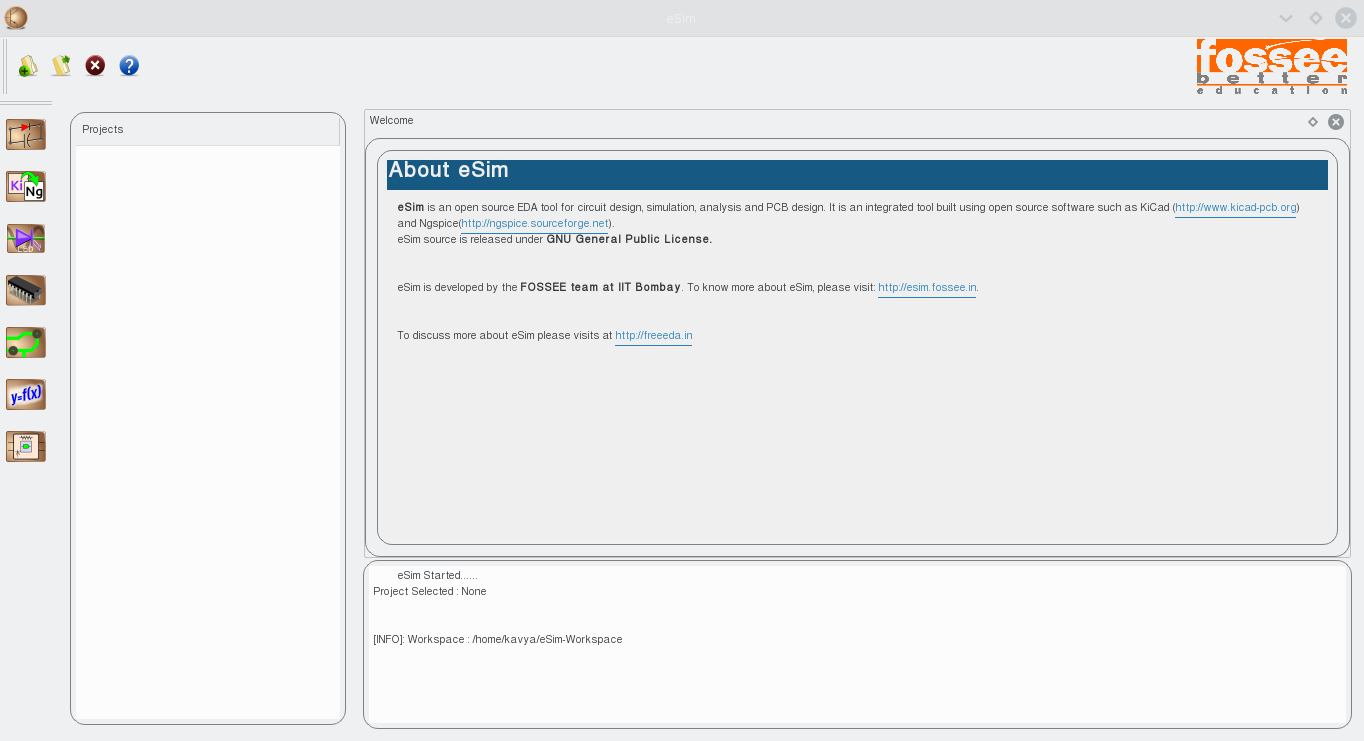
\includegraphics[width=0.8\textwidth]{LaunchWindow.png}
%\caption{Launching eSim will take you to this window}
%\label{LaunchWindow}
%\end{figure}

\subsubsection{Create a New Project}

\paragraph{ } The new project is created by clicking the New icon on the
menubar. The name of the project is given in the pop up window.% as shown in Figure.\ref{newproject}.
%\begin{figure}[h]
%\centering
%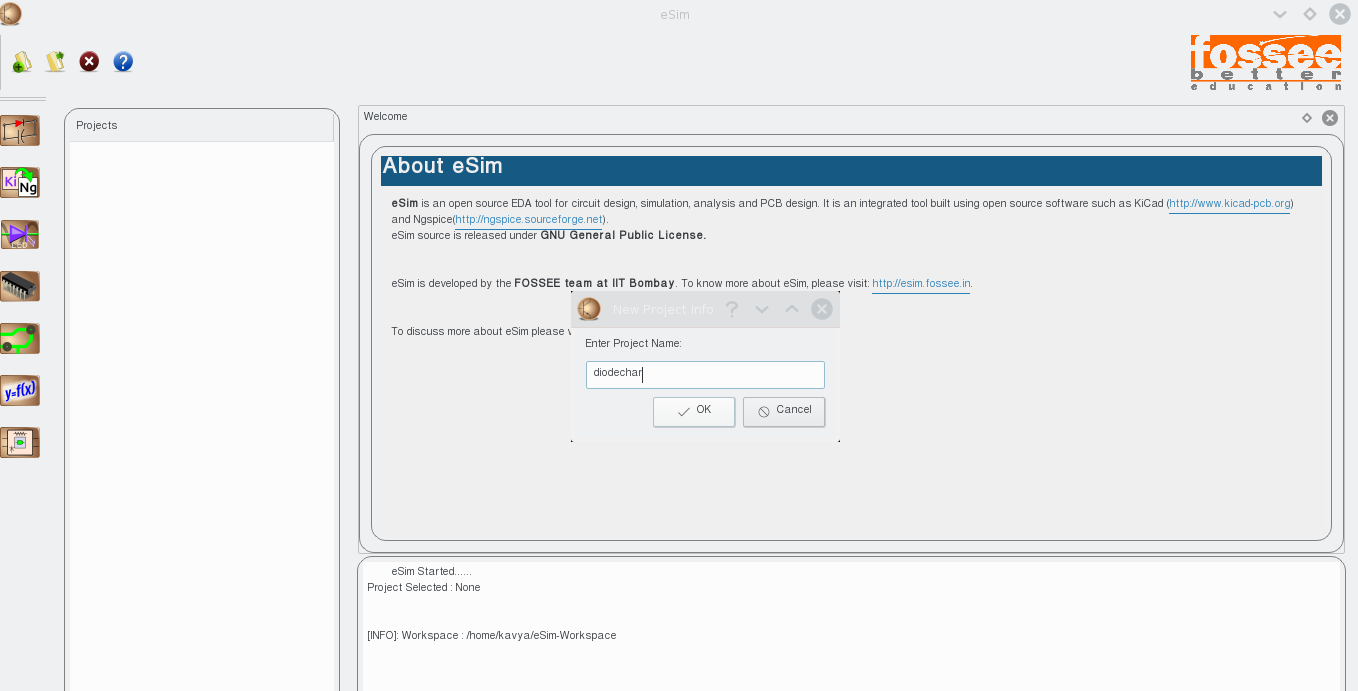
\includegraphics[width=\textwidth]{newproject.png}
%\caption{Creating new project}
%\label{newproject}
%\end{figure}

\subsubsection{Create the Schematic}

\paragraph{}  To create the schematic, click the very first icon of the
left toolbar.% as shown in the Figure \ref{newschematic} .
This will open KiCad Eeschema.


%\begin{figure}[h]
%\centering
%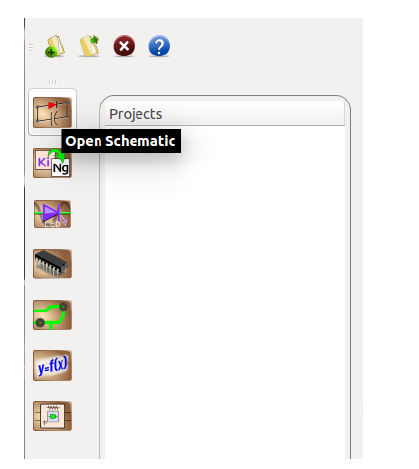
\includegraphics[width=0.5\textwidth, height=6cm]{newschematic.png}
%\caption{Creating new schematic diagram}
%\label{newschematic}
%\end{figure}

To create a schematic in KiCad, we need to place the required components. %See Figure \ref{kicad}

%\begin{figure}[h]
%\centering
%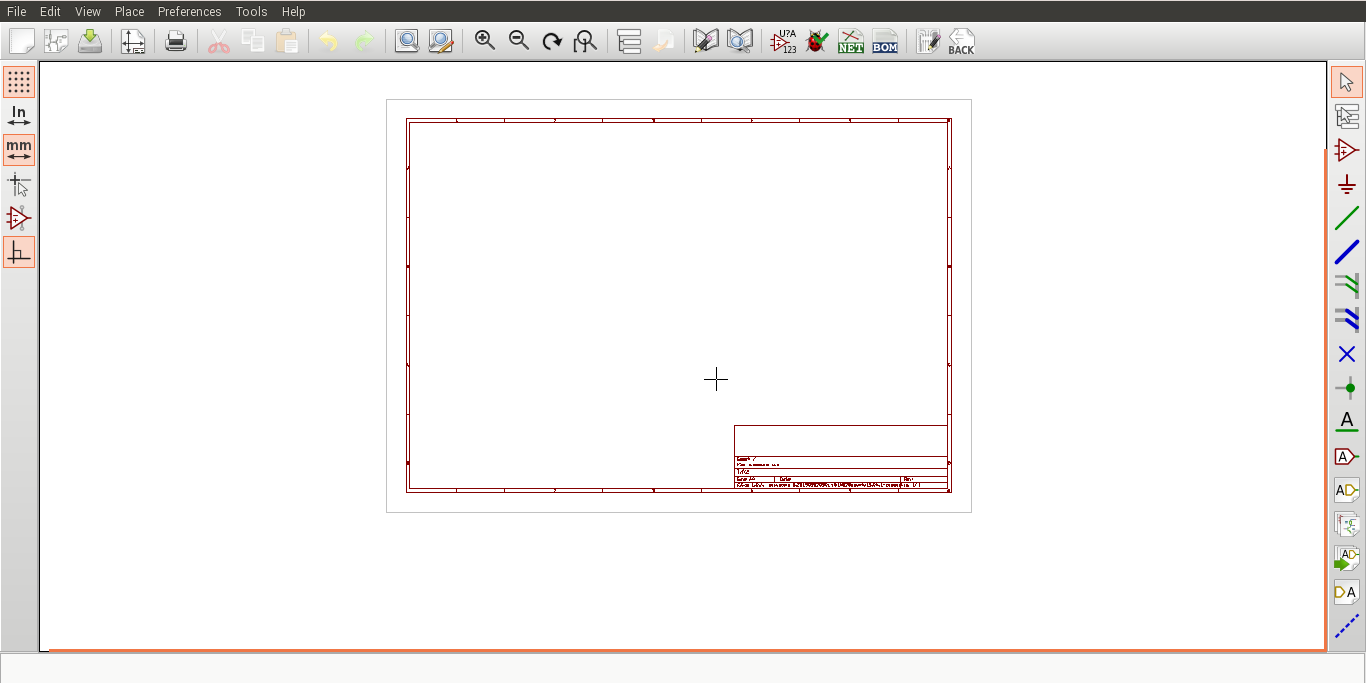
\includegraphics[width=0.5\textwidth, height=6cm]{kicad.png}
%\caption{The Kicad Eeschema page}
%\label{kicad}
%\end{figure}

 Clicking on the icon on the right toolbar opens the component library. After all the required components of the circuit are placed, wiring is
done using the Place Wire option. %as shown in the Figure \ref{placewire}.
 Scroll up and down for zooming in and out.


%\begin{figure}
%\begin{minipage}{.5\textwidth}
%  \centering
%  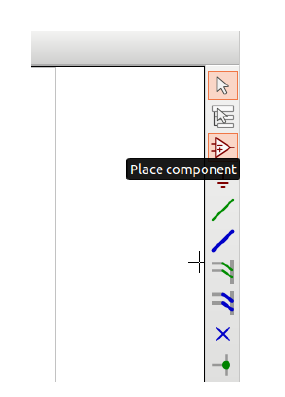
\includegraphics[width=\linewidth]{placecomponent.png}
%  \caption{Place component icon}
%  \label{placecomponent}
%\end{minipage}%
%\begin{minipage}{.5\textwidth}
%  \centering
%  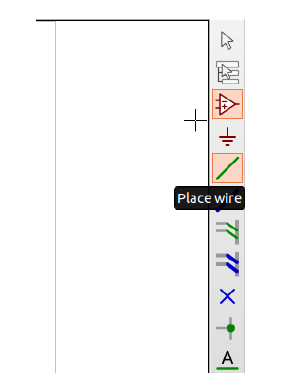
\includegraphics[width=\linewidth]{placewire.png}
%  \caption{Place wire icon}
%  \label{placewire}
%\end{minipage}
%\end{figure}


\paragraph{Placing the Components:} Normally all the components availbale in eSim can be chosen by left mouse click in the grid. The components are listed in different libraries. %See Figure \ref{librarylist}.

%\begin{figure}[h]
%\centering
%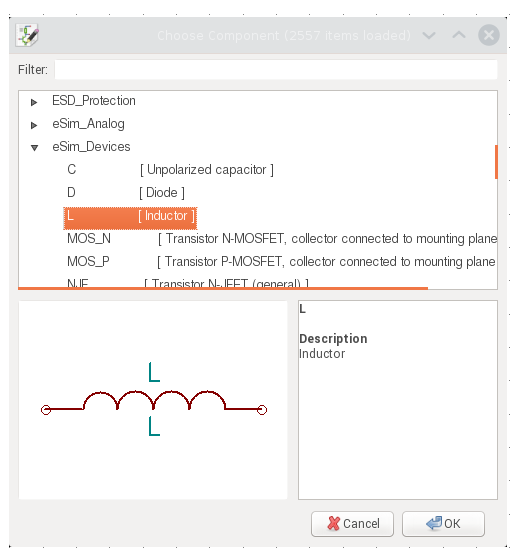
\includegraphics[width=0.5\textwidth, height=4cm]{librarylist.png}
%\caption{The Kicad Libraries of components}
%\label{librarylist}
%\end{figure}

\begin{itemize}
\item
Choose DC sources from eSim\_Sources
\item
Choose resistors from eSim\_Devices
\item
Choose NPN from eSim\_Devices
\item
Choose GND from power
\item
Choose plot\_i2  from eSim\_Plots
\end{itemize}

%Select the resistor and edit its component value to 1k as shown in Figure \ref{editvalue}.

%\begin{figure}[h]
%\centering
%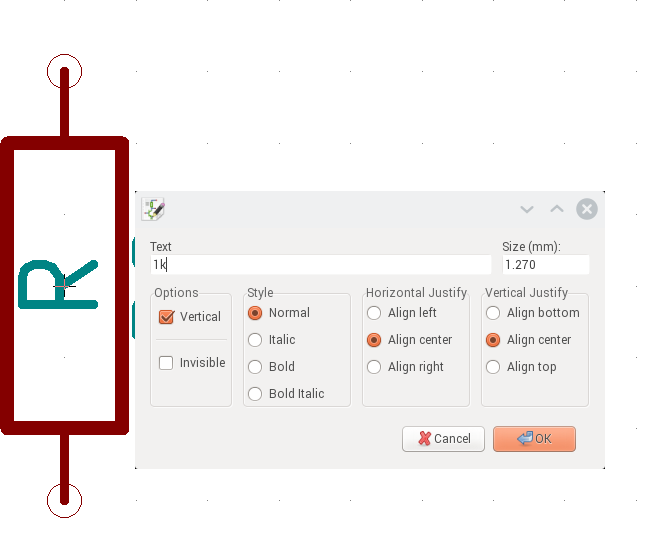
\includegraphics[width=0.5\textwidth, height=6cm]{editvalue.png}
%\caption{Editing the value field of component R}
%\label{editvalue}
%\end{figure}

Wire the components to get the circuit. A global labels `ib' and `vce' have been added to identify the nodes. 
\begin{figure}[h]
\centering
\includegraphics[width=0.8\textwidth]{CEBJTckt1.png}
\caption{Schematic diagram for CE output characteristics}
\label{CEBJTckt1}
\end{figure}

Now we have the circuit diagram as shown in Figure \ref{CEBJTckt1}.


\paragraph{Annotating the circuit:} Once the schematic diagram is completed, annotate it so that the `question marks' associated with the components are converted to meaningful numbers automatically.For that choose annotate button from the top toolbar%(See Figure \ref{toptoolbar} 
and in the subsequenct dialogue boxes appearing click ok and finally close. See Figure \ref{annotation10}.

%\begin{figure}[h]
%\centering
%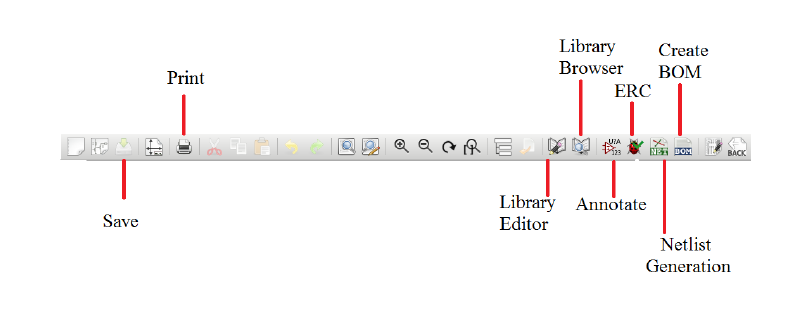
\includegraphics[width=\textwidth, height=4cm]{toptoolbar.png}
%\caption{Choose annotate from the toop tool bar}
%\label{toptoolbar}
%\end{figure}



\paragraph{Note:} If some libraries are found missing, you can add them from the `Preferences` menu by following the procedure: 

\begin{enumerate}
\item
Choose `Component Libraries' from Preferences menu.

\item
Click on the Add button on the top right side of the window.

\item
Choose the required libraries from `user/share/kicad/library' and click OK button

\end{enumerate}

\subsubsection{Create Netlist}

\paragraph{}To simulate the circuit that has been created in the previous section, we need to generate
its netlist. Netlist is a list of components in the schematic along with their connection
information. To do so, click on the Generate netlist tool from the top toolbar. Click on
spice from the window that opens up. Check the option Default Format. Then click
on Generate. Save the netlist. This will be a .cir file. Do
not change the directory while saving.See Figure \ref{createnetlist10}.
 Now the netlist is ready to be simulated. 
\begin{figure}
\begin{minipage}{.5\textwidth}
  \centering
  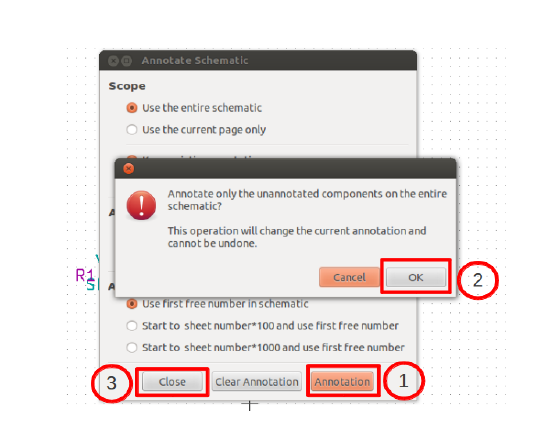
\includegraphics[width=\linewidth]{annotation.png}
  \caption{Annotation}
  \label{annotation10}
\end{minipage}%
\begin{minipage}{.5\textwidth}
  \centering
  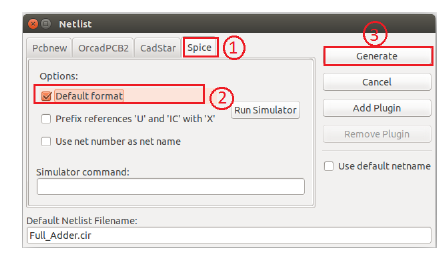
\includegraphics[width=\linewidth]{createnetlist.png}
  \caption{Netlist Generation}
  \label{createnetlist10}
\end{minipage}
\end{figure}

\subsubsection{KiCad to Ngspice conversion}

\paragraph{} To convert KiCad netlist of the circuit to NgSpice
compatible netlist click on KiCad to Ngspice icon as shown in Figure \ref{kcd2spice10}. Now you can choose the type of analysis, source details, device models ngspice models and subcircuit models.


\begin{figure}[h]
\centering
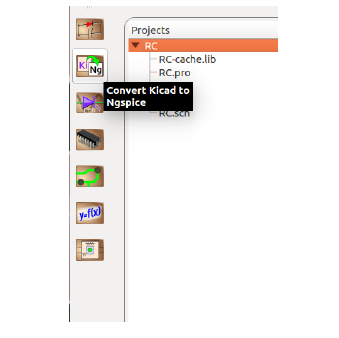
\includegraphics[width=0.5\textwidth, height=4cm]{kcd2spice.png}
\caption{Choose Kicad to Ngspice tool}
\label{kcd2spice10}
\end{figure}


\paragraph{Analysis:}Choose DC analysis type. Choose the values of two DC sources, V1 and I1 in the netlist properly as described below. Change V1 from 0V to 5V at an interval of 0.05V. I1 is to be changed from 0 mA to 5 mA at an increment of 1 mA. See Figure \ref{CEBJTanalysis}


\begin{figure}[h]
\centering
\includegraphics[width=\textwidth, height=4cm]{CEBJTanalysis.png}
\caption{Choose DC analysis type and enter the values of V1 and I1}
\label{CEBJTanalysis}
\end{figure}

\paragraph{Source:} Give the details of source as in Figure \ref{CEBJTsource}.

\begin{figure}[h]
\centering
\includegraphics[width=\textwidth, height=4cm]{CEBJTsource.png}
\caption{GiveSource Details of V1 and I1}
\label{CEBJTsource}
\end{figure}

\paragraph{Ngspice Model:} No Ngspice model to be given.

\paragraph{Device Model:} The NPN transistor is a device whose model details must be given for simulation. Let us choose the generic NPN model availabe in the eSim model library. Browse it from \texttt{/opt/eSim/src/deviceModelLibrary/Transistor/NPN.lib}. See Figure \ref{NPNmodel1}.

\begin{figure}[h]
\centering
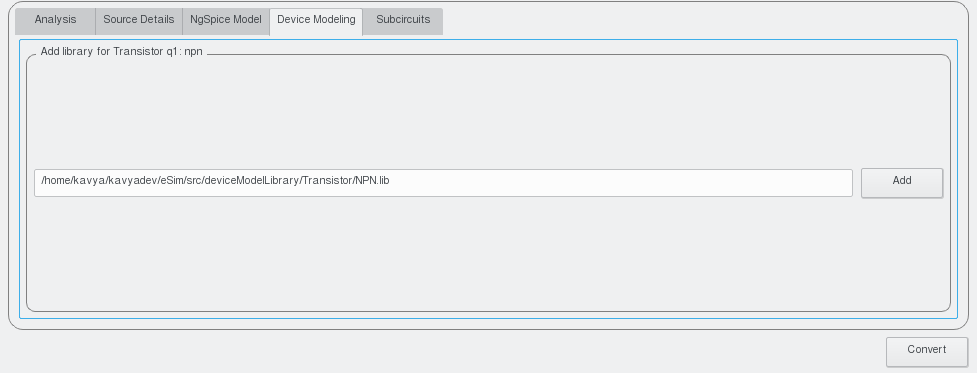
\includegraphics[width=\textwidth, height=6cm]{NPNmodel.png}
\caption{Choose the required NPN model}
\label{NPNmodel1}
\end{figure}

\paragraph{Subcircuits:} No subcircuits to be given.

\paragraph{}
 Once these details are provided click on convert button. %See Figure \ref{diodemodel}. 
Now you are ready to see the simulation results.

\subsubsection{Simulate} To run Ngspice simulation click the simulation icon in the left tool bar. Since we have used plot components, the required output characteristic plots will automatically pop-up as shown in Figure. \ref{CEBJToutput}


\begin{figure}[h]
\centering
\includegraphics[width=12cm, height=6cm]{CEBJToutput.png}
\caption{The output characteristics of NPN transistor }
\label{CEBJToutput}
\end{figure}
%\begin{figure}[h]
%\centering
%\includegraphics[width=12cm, height=6cm]{MOSFETdrain1.png}
%\caption{The drain characteristics of MOSFET with gate voltage =1V }
%\label{MOSFETdrain1}
%\end{figure}


\section*{RESULT}
The circuit for plotting the common emitter charateristics of NPN transistor was implemented and simulated.


